\documentclass{article}

\usepackage[UTF8]{ctex}
\usepackage{amsmath,amssymb}
\usepackage{geometry}
\usepackage{graphicx}

\geometry{a4paper, margin=2.5cm}
\setlength{\emergencystretch}{1em}

\begin{document}

% ============================================================
\section*{从偏好到奖励（RLHF / Reinforcement Learning from Human Feedback）}

\subsection*{先讲一个故事}

你想让一个语言模型「回答得更好」。好，意味着准确、克制、有帮助、不胡编——你试着把这些写成一个奖励函数，很快就会放弃：这些标准既写不全，也写不准。

\textbf{错误做法 / 朴素做法}：手工设计打分规则——回答越长加分、出现礼貌用语加分、命中关键词加分。模型会立刻学会刷规则：无限拉长回答、堆砌客套话，分数很高，回答很差。

\textbf{本章方法的做法}：不定义「好」，而是让人\textbf{比较}——同一个问题的两个回答，哪个更好？从大量成对比较中学出一个\textbf{奖励模型}，再用强化学习（第 7 章的 PPO）去优化它。

\textbf{本章的核心问题}：学出来的奖励只是真实偏好的\textbf{代理}，它能被优化多远而不被击穿？

\[
\boxed{\max_{\pi}\; \mathbb{E}_{y\sim\pi}\left[r_{\varphi}(y)\right] - \beta\,\mathrm{KL}\!\left(\pi \,\|\, \pi_{\mathrm{ref}}\right)}
\]

\subsection*{数学形式化}

偏好数据是成对比较：给定两个候选 $y_a, y_b$，标注者选出更好的一个。Bradley--Terry 模型假设比较概率由潜在奖励之差决定：

\[
\boxed{P(y_a \succ y_b) = \sigma\!\left(r_{\varphi}(y_a) - r_{\varphi}(y_b)\right)}
\]

\begin{itemize}
  \item $r_{\varphi}$ —— 奖励模型，从偏好对中学习，是真实偏好的代理；
  \item $\pi_{\mathrm{ref}}$ —— 参考策略（通常是 SFT 模型），偏好数据从它的样本中采集；
  \item $\beta$ —— KL 锚定系数，控制策略离参考策略多远；
  \item $\sigma$ —— sigmoid 函数，把奖励差映射为比较概率。
\end{itemize}

% ============================================================
\section*{奖励从哪里来：偏好建模}

\subsection*{Bradley--Terry 负对数似然}

给定偏好对集合 $\{(y_w, y_l)\}$（$y_w$ 胜、$y_l$ 负），奖励模型通过最小化负对数似然学习：

\[
\boxed{\mathcal{L}(\varphi) = -\,\mathbb{E}_{(y_w, y_l)}\left[\log \sigma\!\left(r_{\varphi}(y_w) - r_{\varphi}(y_l)\right)\right]}
\]

注意 BT 模型只由\textbf{奖励差}决定：给 $r_{\varphi}$ 整体加一个常数，似然不变（平移不变）；而整体尺度由数据中偏好翻转的比例隐式决定，不同种子、不同数据量下学到的尺度并不稳定。因此奖励的绝对数值没有可比性，实践中先在参考分布上做\textbf{白化}（减均值、除标准差）再交给 RL——这也让 $\beta$ 在不同种子、不同任务间可迁移。

\subsection*{奖励只在数据覆盖区内可信}

偏好对从参考策略的样本中采集，奖励模型因此只在\textbf{参考策略的样本分布}上被约束过。覆盖区之外它照样输出数值——但那是网络归纳偏置的外推，不是学到的知识：ReLU 网络在训练支撑集外按分段线性规律\textbf{线性外推}，会把「适量有益」外推成「越多越好」。

这与第 9 章离线强化学习的处境完全同构：价值函数（那里是 $Q$，这里是 $r_{\varphi}$）在数据支撑外的估计没有依据，一旦有一个优化器专门去寻找高估的方向，错误就会被无限放大。

实验用一个完全合成的序列任务把这件事摆到明面上：真实质量等于 token 价值均值加上「强调 token」的凹形加分——每个加 $0.3$ 分，超过 $3$ 个后每个倒扣 $0.6$ 分；参考策略几乎不产生超过 $3$ 个强调 token 的序列，偏好数据只覆盖加分的上升段。图~1 左侧显示验证集偏好精度随数据量稳定上升（$0.82 \to 0.86$）；右侧显示覆盖区内奖励模型与真实分数一致，覆盖区外真实分数见顶崩坏、奖励模型继续单调上扬。

\begin{figure}[!htbp]
  \centering
  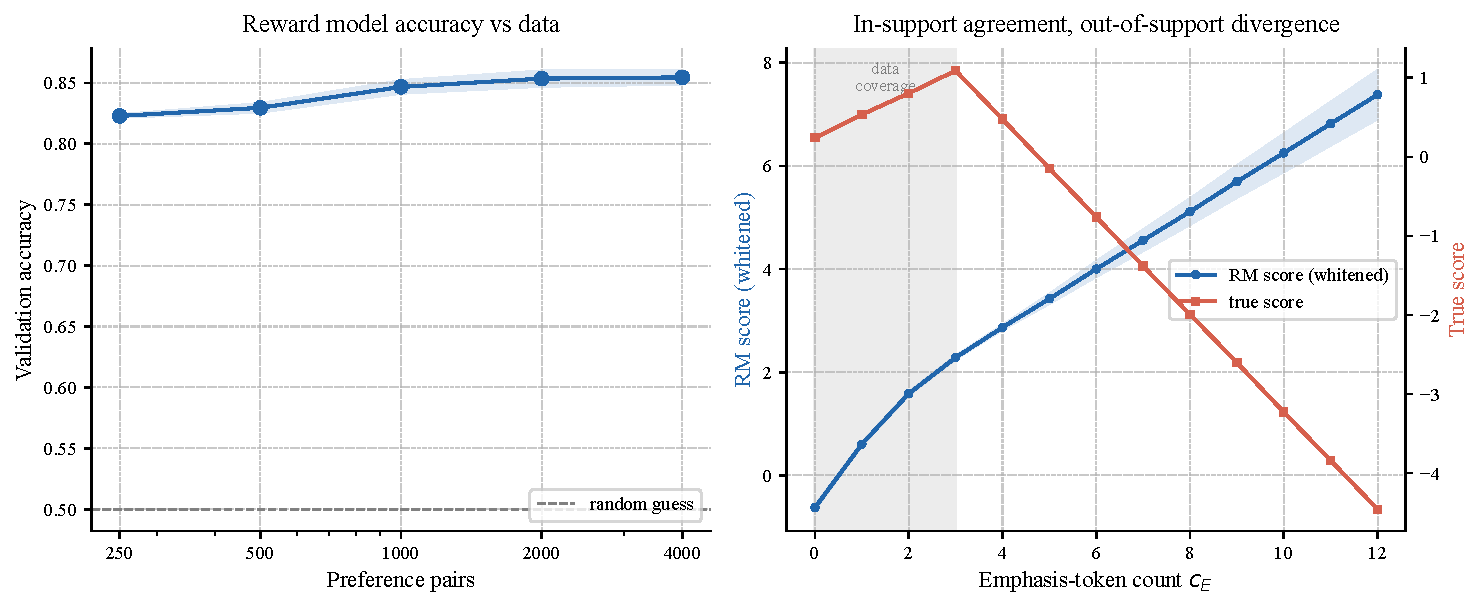
\includegraphics[width=0.88\textwidth]{fig1_reward_model.pdf}
  \caption{奖励模型的可信边界（玩具序列任务，3 个随机种子，阴影为 $\pm 1\sigma$）。左：验证集偏好精度随偏好对数量上升；右：偏好数据覆盖区（灰色，$c_E \le 3$）内奖励模型与真实分数一致，覆盖区外真实分数在 $c_E=3$ 见顶后崩坏，而奖励模型继续单调外推——分叉处就是 reward hacking 的入口。}
  \label{fig:rlhf-rm}
\end{figure}

% ============================================================
\section*{核心机制}

\subsection*{机制一：Reward hacking——优化器专找分叉}

Goodhart 定律：\textbf{当一个度量成为优化目标，它就不再是好度量}。PPO 不知道什么是「真实质量」，它只会沿代理奖励最陡的方向爬——而奖励模型给出的最陡方向，恰恰通向它自己没有依据的外推区。

图~2 是 $\beta=0$（无 KL 锚定）的完整轨迹：约前 30 轮是\textbf{真实提升}（真实分数从 $+0.39$ 升到约 $+1.0$，策略把强调 token 用到甜点区附近）；随后优化冲出数据覆盖区，把强调 token 打满——代理奖励继续上涨到 $+7$ 以上，真实分数崩塌到 $-4.5$。代理指标一路向好、真实目标一路崩坏，与第 9 章「Q 涨、回报跌」是同一张图的两个化身。

\begin{figure}[!htbp]
  \centering
  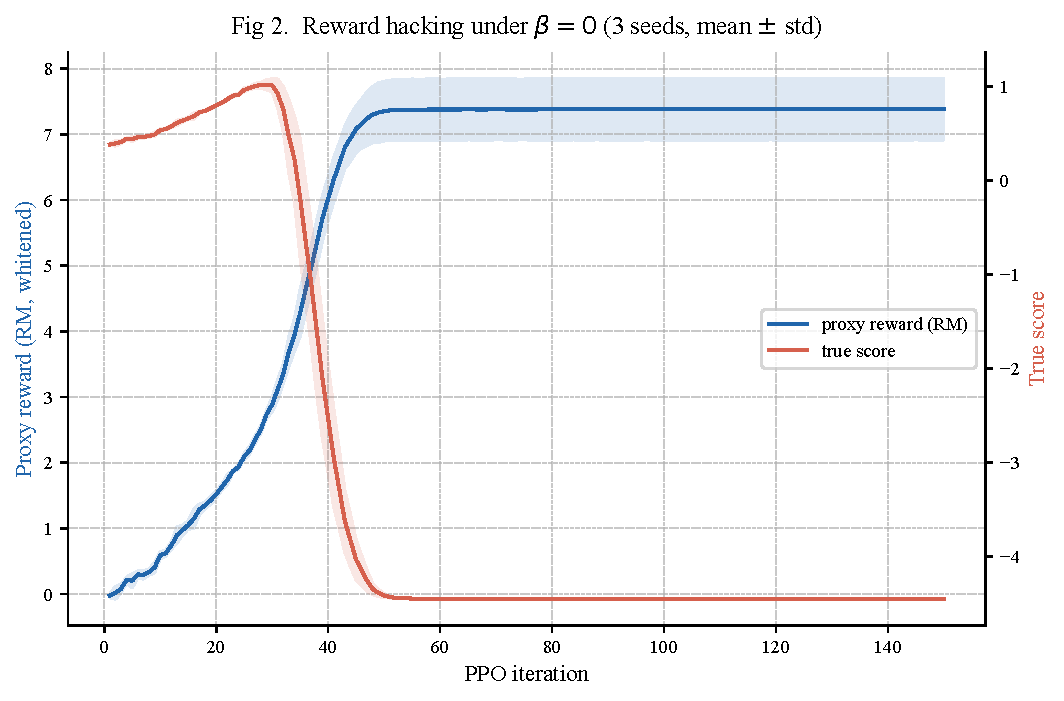
\includegraphics[width=0.88\textwidth]{fig2_reward_hacking.pdf}
  \caption{$\beta=0$ 时的 reward hacking（3 个随机种子，阴影为 $\pm 1\sigma$）。约前 30 轮为真实提升（真实分数 $+0.39 \to$ 约 $+1.0$）；随后策略冲出偏好数据覆盖区，代理奖励（左轴）继续上涨到 $+7$ 以上，真实分数（右轴）崩塌到 $-4.5$。}
  \label{fig:rlhf-hacking}
\end{figure}

\subsection*{机制二：KL 锚定——把优化关在可信区附近}

解药不是修好奖励模型（它在覆盖区外注定不可信），而是\textbf{不让策略走出覆盖区太远}。在目标中加入对参考策略的 KL 惩罚：

\[
\boxed{J(\pi) = \mathbb{E}_{y\sim\pi}\left[r_{\varphi}(y)\right] - \beta\,\mathrm{KL}\!\left(\pi \,\|\, \pi_{\mathrm{ref}}\right)}
\]

KL 项把策略拴在参考策略的邻域内，而奖励模型恰好在这个邻域内被数据约束过——两者的「可信区」是同一个区域，这不是巧合，而是 KL 锚定有效的根本原因。

$\beta$ 是一个真正的权衡超参。图~3 给出三种结局：$\beta=0$ 崩塌；$\beta=0.5$ 把最终 KL 压在约 $2$ nats，真实分数稳定在约 $+0.84$ 的真提升区；$\beta=2.0$ 锚定过强，策略几乎钉在 SFT 水平（约 $+0.53$），浪费了偏好信息。

\begin{figure}[!htbp]
  \centering
  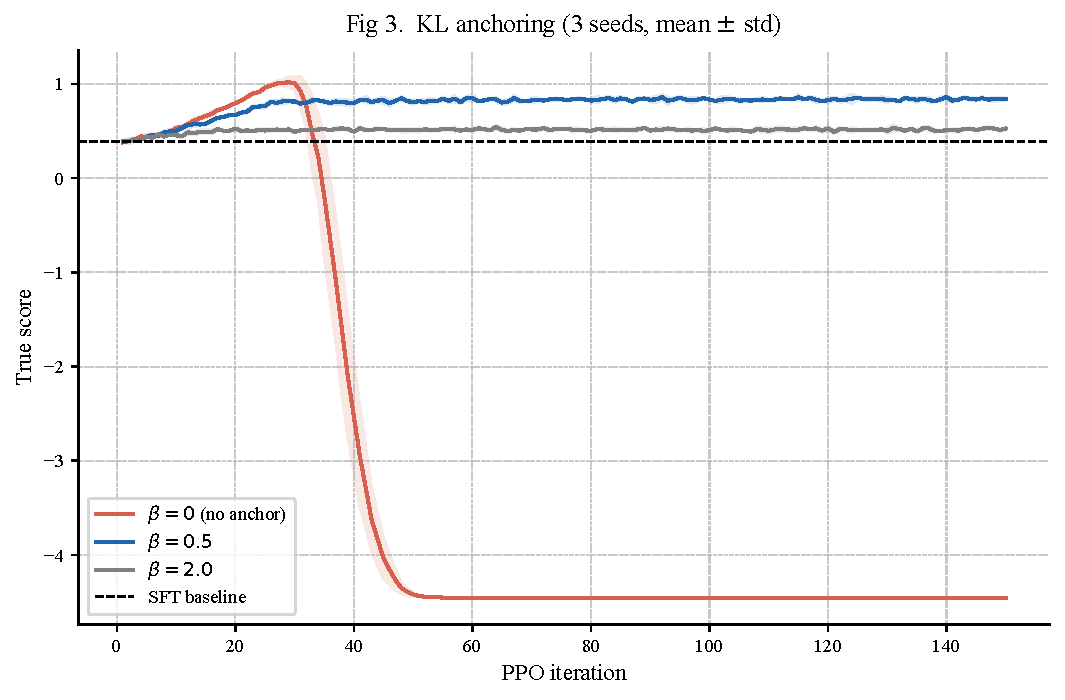
\includegraphics[width=0.88\textwidth]{fig3_kl_anchor.pdf}
  \caption{KL 锚定的三种结局（3 个随机种子，阴影为 $\pm 1\sigma$，虚线为 SFT 基线 $+0.39$）。$\beta=0$ 崩塌到 $-4.5$；$\beta=0.5$ 稳定在约 $+0.84$（最终 KL 约 $2$ nats）；$\beta=2.0$ 锚定过强，几乎钉在 SFT 水平（约 $+0.53$）。}
  \label{fig:rlhf-kl}
\end{figure}

\subsection*{机制三：奖励白化——让 $\beta$ 有稳定的量纲}

BT 似然对奖励的平移和缩放不变，不同训练得到的奖励模型天然处在不同尺度上。若直接把原始分数交给 RL，同一个 $\beta$ 在不同种子间的实际约束强度会相差数倍。在参考分布上白化（$\tilde{r} = (r - \mu_{\mathrm{ref}})/\sigma_{\mathrm{ref}}$）后，「奖励一个标准差」与「KL 一个 nat」之间的兑换率才是稳定的。

% ============================================================
\section*{完整算法流程}

\subsection*{RLHF 四步}

\begin{enumerate}
  \item \textbf{SFT}：在示范数据上监督微调，得到参考策略 $\pi_{\mathrm{ref}}$；
  \item \textbf{偏好收集}：从 $\pi_{\mathrm{ref}}$ 采样成对候选，由标注者比较；
  \item \textbf{奖励建模}：用 BT 负对数似然训练 $r_{\varphi}$，在参考分布上白化；
  \item \textbf{RL 微调}：用 PPO 最大化 $\tilde{r}_{\varphi} - \beta\,\mathrm{KL}$，必要时回到第 2 步用新策略的样本迭代扩充偏好数据。
\end{enumerate}

% ============================================================
\section*{与相邻方法对比}

\subsection*{RLHF vs SFT，以及与离线 RL 的同构}

\begin{itemize}
  \item \textbf{SFT} 模仿数据的平均行为，无法超过示范水平；\textbf{RLHF} 沿偏好方向优化，可以超过示范——代价是引入可被击穿的代理奖励；
  \item \textbf{与离线 RL 同构}：第 9 章里 $\max$ 算子放大 $Q$ 在数据外的高估，本章里 PPO 放大 $r_{\varphi}$ 在覆盖区外的外推——同一个病（数据支撑外的乐观估计被优化器放大），CQL/IQL 把悲观写进价值或动作集合，RLHF 把约束写进 KL 项。
\end{itemize}

% ============================================================
\section*{本章在 RL 体系中的位置}

\begin{enumerate}
  \item 上游：PPO（第 7 章）提供优化引擎；离线强化学习（第 9 章）提供「外推误差被优化放大」的病理模型；
  \item \underline{从偏好到奖励（RLHF）}（本章：当奖励本身也要学习时，优化的边界由数据覆盖决定）；
  \item 下游：DPO 绕开显式奖励模型，把偏好直接写进策略目标；GRPO 与可验证奖励（RLVR）用规则奖励替代学习奖励，消除被击穿的可能。
\end{enumerate}

读者应带走一句话：\textbf{学出来的奖励是一张有边界的地图，RL 是一辆没有刹车的车——KL 锚定不是让地图变准，而是不让车开出地图}。下一章从 DPO 开始，看如何不画这张地图。

\subsection*{参考资料}

\small
\begin{enumerate}
  \item Christiano et al.\ (2017). Deep Reinforcement Learning from Human Preferences. \textit{NeurIPS}.
  \item Ziegler et al.\ (2019). Fine-Tuning Language Models from Human Preferences.\allowbreak\ \textit{arXiv:1909.08593}.
  \item Stiennon et al.\ (2020). Learning to Summarize with Human Feedback.\allowbreak\ \textit{NeurIPS}.
  \item Ouyang et al.\ (2022). Training Language Models to Follow Instructions with Human Feedback. \textit{NeurIPS}.
  \item Gao, Schulman \& Hilton (2023). Scaling Laws for Reward Model Overoptimization. \textit{ICML}.
\end{enumerate}

\end{document}
